\chapter{METODOLOGIA}
\thispagestyle{empty}

O projeto presente tem por finalidade analisar a efetividade da gestão de projetos em um escritório de projetos de um polo de inovação identificando a maturidade destes projetos através do mapeamento deste escritório sob um modelo de maturidade proposto pela EMBRAPII, e um modelo mundialmente usado por profissionais de GP. Neste contexto, este capítulo descreverá sobre a metodologia a ser utilizada.


\section{A natureza de pesquisa}

Esta pesquisa pode ser caracterizada como uma pesquisa bibliográfica, cujo método utilizado foi o estudo de caso. Visando atingir o objetivo da pesquisa, inicialmente, foi realizada uma pesquisa bibliográfica através do material existente na literatura.

Através da leitura foi possível identificar os elementos de pesquisa propostos por \citeonline{lakatos2010fundamentos}, são eles: intenção, reflexão, espírito crítico, atenção, análise e síntese.

Se utilizada a proposta de \citeonline{gil2002elaborar}, a presente pesquisa é tomada por qualitativa quanto a abordagem da problemática, e descritiva quanto a caracterização de seus objetivos, pois utiliza do desenvolvimento de um estudo de caso.

\citeonline[p 239]{fortin2009fundamentos} confirma que todo estudo que objetiva a identificação de características referentes a um fenômeno, visando obter uma visão geral de sua situação ou população em questão, pode ser apresentado como um estudo descritivo. Nestas condições, determinado trabalho consistirá na pretenção de descrever ou interpretar a propriedades desta investigação, através de análises empíricas e da descrição da problemática \cite{fortin2009fundamentos, lakatos2010fundamentos}.

\section{Método de Pesquisa}

Para \citeonline{de2007metodologia} todo e qualquer trabalho científico deve proporcionar a reprodução de experiências de modo que outros pesquisadores sejam capazes de obter resultados descritivos, de repetir suas observações e ainda de realizar julgamentos as conclusões de seu(s) autor(es).

De acordo com \citeonline{vergara2009projetos} pesquisas também podem ser caracterizadas em relação aos aspectos relativos aos fins e aos meios. A presente pesquisa apresenta influência no caráter exploratório descritivo quanto aos fins, pois teve como objetivo \'analisar a efetividade da gestão de projetos em um escritório de projetos de um polo de inovação \'e se propõe a expor características de uma determinada população, sem o compromisso de explicar os fenômenos que descreve, embora sirva de base para essa explicação.

Quanto aos meios, a pesquisa classifica-se como bibliográfica e de campo.

Assim, porque é de pretensão deste trabalho descrever e interpretar, mais do que avaliar um caso real presente, e seguindo o caráter de investigação revelado por \citeonline{fortin2009fundamentos}, este trabalho se apresenta como descritivo e exploratório.

Por sua vez, quanto aos procedimentos técnicos que foram utilizados para obtenção dos dados, seguindo a classificação proposta por \citeonline{lakatos2010fundamentos}, trata-se de pesquisa bibliográfica, que também pretende utilizar de uma pesquisa de campo. Uma pesquisa de campo é aquela que busca alcançar informações referentes a um problema e busca uma resposta ou de uma hipótese, que se pretende comprovar, bem como descobrir novos fenômenos ou as relações entre eles \cite{de2007metodologia}.


\section{População e Amostragem}

  \citeonline[p 20]{de2011elaboraccao} define população de pesquisa como aqueles a quem ela se refere ou representa, isto é, o universo compreendido dentro da pesquisa. Nesta pesquisa, o universo abordado se refere aos funcionários envolvidos no processo de formação do escritório de projetos do PICG, dentro do contexto de gestão de projetos.

  Segundo \citeonline{embrapii2013}, a Associação Brasileira de Pesquisa e Inovação Industrial (EMBRAPII) é qualificada como uma Organização Social, fundada em setembro de 2013, sob reconhecimento da capacidade de inovação brasileira via exploração da sinergia entre instituições de pesquisa tecnológica e empresas industriais. Sua missão é contribuir para o desenvolvimento da inovação na indústria através do fortalecimento de instuições de pesquisa tecnológicas, em selecionadas áreas de competência.

  O Polo de Inovação Campos dos Goytacazes (PICG), conhecido até então por Unidade de Pesquisa e Extensão Agroambiental (UPEA) no momento em que foi inaugurado em outubro de 2007, foi criado no intuito de possibilitar o desenvolvimento de atividades de Pesquisa, Desenvolvimento e Inovação (P\&DI) associadas ao Instituto Federal Fluminense (IFF). Desde sua criação, a unidade realiza atividades de PD\&I, notadamente na área ambiental, em atendimento de demandas regionais, a partir de parcerias com empresas  órgãos de governo. Assim, em agosto de 2015, o PICG foi oficialmente reconhecido por integrar uma unidade EMBRAPII de Monitoramento e Intrumentação para o Ambiente \cite{embrapiiff}.

  Este polo é também responsável pela formação de recursos humanos, via programa de capacitação desenvolvido na sede do Centro de Referência para profissionais de empresas parceiras, servidores, estudantes e responsáveis pela execução dos projetos. Além da capacitação técnica, o programa se responsabiliza pela gestão atual e a longo prazo, ampliando, dessa forma, as possibilidades do Polo de atender as solicitações das indústrias.

  No momento de parceria entre a EMBRAPII e o PICG, foi estabelecido um modelo de financiamento que prevê ao polo autonomia de atuação, sob responsabilidade exclusiva de execução dos projetos, aplicação dos recursos financeiros e de prestação de contas. Neste modelo também foi estabelecido que os resultados, ou entregas, dos projetos seriam qualificados quanto ao nível de maturidade tecnológica do modelo EMBRAPII, sendo sempre necessário que os níveis estivessem considerados entre três e seis desta escala \cite{iffembrapii2016}.

  Para atender a discussão científica proposta no presente estudo, de acordo com a posição de \citeonline{vergara2009projetos}, foi apresentada uma problemática referente ao universo que será exposta no próximo capítulo.

% \section{Limitações dos Métodos de Pesquisa}

\section{Modelo de Excelência Operacional EMBRAPII}

  De acordo com \citeonline{embrapii_sistema} um produto tecnologicamente inovador precisa de mais do que conhecimento técnico para estar apto a ser lançado e ter sucesso comercial. Entre as muitas competências necessárias é preciso considerar seus desafios de produção, implatação e ainda seu impacto no mercado.

  Para definir bases que orientem os polos de inovação na fase pré-competitiva da inovação tecnológica industrial nos projeto de Pesquisa e Desenvolvimento (P\&D), a EMBRAPII apresenta um padrão de referência de mensuração para avaliar o nível de maturidade tecnológica de cada projeto. Este padrão, que pode ser referido por Sistema de Excelência Operacional EMBRAPII (EOE), foi baseado no modelo, amplamente empregado, \textit{Technology Readiness Level} (TRL), juntamente com uma base na norma ISO 16290:2013 \cite{embrapii_manual}.

  Além de um padrão, o EOE serve de referência para os sistemas de gestão de todas as Unidades EMBRAPII (UE), com a finalidade de contribuir para a realização dos objetivos do sistema EMBRAPII. Entre estes objetivos, são especificados \cite{embrapii_sistema}:

  \begin{itemize}
    \item Descrever os processos de negócio e os componentes de um modelo de gestão;
    \item Orientar a UE sobre o desenvolvimento contínuo de conhecimentos na área de sua competência para garantir o papel de indutor da tecnologia;
    \item Apoiar o EOE nos processos de qualificação e acompanhamento das suas UE.
  \end{itemize}

  Em sua elaboração, o sistema EOE considerou, além das normas, algumas diretrizes que o auxiliam a atender alguns requisitos como:

  \begin{itemize}
    \item \textbf{Complementaridade:} presupõe-se que a UE passui uma área de competência claramente focada e experiência prévia com inovação tecnológica, e um sistema de gestão da qualidade minimamente constituído para que o EOE não tenha o papel de substituir este sistema, mas sim de promover a complementaridade, padronização e adequação dos sistemas de gestão existentes;
    \item \textbf{Referência para busca contínua da excelência:} não é objetivada a explicação sobre como cada passo deve ser procedido, a forma de operacionalizar as práticas propostas fica a cargo de cada UE;
    \item \textbf{Evidências de melhores práticas:} cada instrução e componente foram extraídos de recomendações consagradas nas áreas de gestão de tecnologia, gestão de projetos, gestão de desenvolvimento de produtos e gestão da inovação;
    \item \textbf{Simplicidade:} optou-se pela menor quantidade possível de conceitos, elementos, processos e técnicas, com o interesse de manter um modelo de gestão simplificado e eficiente;
    \item \textbf{Experiência:} foram consideradas experiências do projeto piloto EMBRAPII e de outras iniciativas para garantir a efetividade proposta;
    \item \textbf{Melhoria contínua:} entende-se que cada versão do sistema EOE deverá ser continuamente atualizada.
  \end{itemize}

  Este padrão se utiliza de uma classificação estabelecida em níveis de 1 a 9, com base da observação de parâmetros atribuídos aos projetos, onde cada projeto pode ser constituído por uma nova ideia, um conceito, um achado científico, um produto/processo ou ainda uma forma de integração a um sistema existente e inovador.

  Na Figura~\ref{niveis_embrapii} esta ilustrada a escala de classificação desta norma.

  \begin{figure}[!h]
    \centering
    \scalebox{0.6}{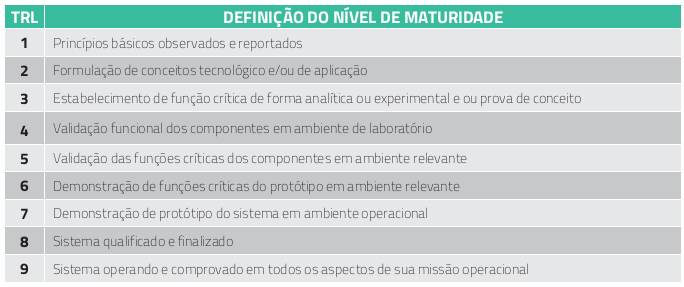
\includegraphics{figuras/niveis_embrapii}}
    \caption{Escala de classificação do padrão EMBRAPII. Fonte: \cite{embrapii_manual}}
    \label{niveis_embrapii}
  \end{figure}

  Para que estejam no âmbito EMBRAPII todos os resultados ou entregas, dos projetos de Pesquisa Desenvolvimento e Inovação (PD\&I) contratados, devem estar estabelecidos na escala de 3 a 6 dos níveis de maturidade tecnológica deste padrão.

  No que respeito a sua contribuição para a excelência operacional, em todas as UE, o EOE se sustenta em meio a três pilares \cite{embrapii_sistema}:

  \begin{itemize}
    \item \textbf{Demanda tecnológica:} Este pilar indica que uma vez identificada uma demanda empresarial,o seu atendimento deve ser realizado de maneira rápida, eficiente e assertiva.
    \item \textbf{Indução tecnológica:} pilar da indução tecnológica indica que o papel da UE não pode ser unicamente reativo, isso é, apenas atender ao que é demandado pela empresa. Espera-se que cada Unidade ofereça as mais atuais soluções para os desafios apresentados pela empresa, com base na experiência da UE com outros projetos e resultados práticos.
    \item \textbf{Geração de competências:} A UE deve ainda possuir uma ação efetiva de planejamento e desenvolvimento de novos conhecimentos em sua área de competência para garantir que os pilares de demanda e indução tecnológica sejam sustentados no longo prazo, acompanhando o avanço tecnológico em sua área de atuação.
  \end{itemize}
